\section{Algorithm execution}
\label{sec-algorithm-execution}

\textbf{Created by:} Milos Drobnjakovic \\
\textbf{Modified by:} Milos Drobnjakovic \\

\subsection*{Scenario Objective}

This scenario depicts how to express executions of algorithms by using BFO/IOF ontology.

Specifically, this pattern focuses on algorithm executions which produce Information Content Entities (ICEs) as outputs. As such, algorithms that return no ‘outputs’ are not included in this pattern.

This scenario is limited to algorithms that are part of a software system.


\subsection*{General Pattern Description}
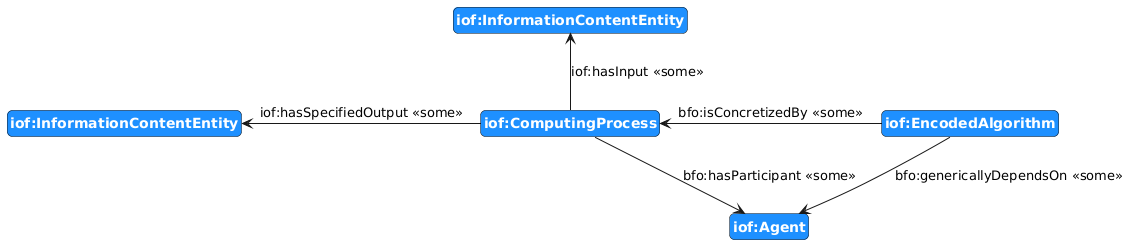
\includegraphics[scale=0.6]{scenarios/algorithm-execution/images/algorithm-execution-general.png}

...

\subsubsection*{Use Case: Drill failure prediction} 
A multilayer perceptron (MLP – a type of a neural network) is used to predict drill failure based on five measured parameters: ‘tool wear’, ‘air temperature’, ‘process temperature’, ‘torque’,’rotational speed’. The model uses the given parameters and outputs either ‘FAIL’ or ‘NOT FAIL’.

\subsubsection*{Use-Case Pattern Description}

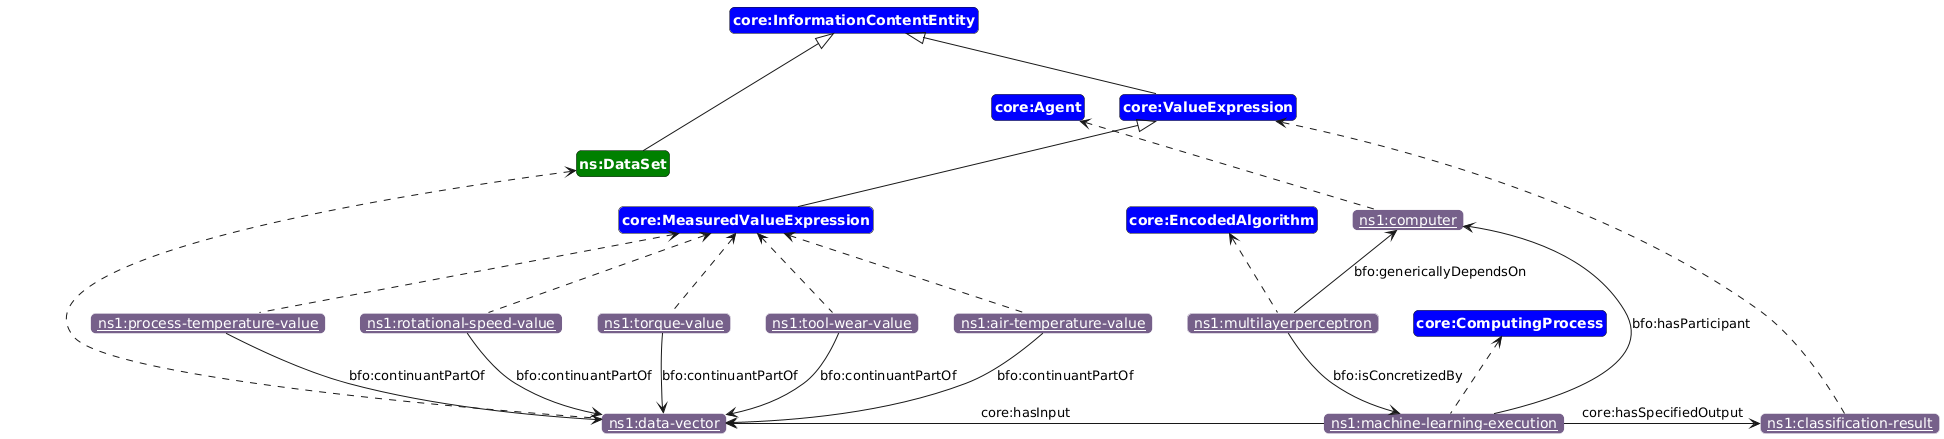
\includegraphics[scale=0.23]{scenarios/algorithm-execution/images/algorithm-execution-usecase1.png}

The machine learning model (MultiLayerPerceptron1) - an instance of:Encoded Algorithm is being concretized in a model execution process - an instance of:Computing Process. The MLP generically depends on a computer system (in this case an instance of Agent) which participates in the model execution process. Model execution utilizes the measured values associated with the drill and the drilling process and produces a ClassificationResult which is an instance of a ValueExpression. Since the objective is to predict machine failure the ClassificationResult is a prediction of the DrillFunction. The ClassificationResult can have two values associated with hasSimpleExpressionValue: 1) FAIL or 2) NOT FAIL. On the diagram bellow an example with the FAIL value is given. For brevity purposes the actual measurement values and their units are excluded from the diagram. Also, the association of the measured values with “drill attributes” or the “drilling process” are omitted. For a detailed guide on connecting the measured values with different entties - the user should see (placeholder link).

\subsubsection*{Use-Case Example Data}

For this use case a publicly available dataset was used: Predictive Maintenance⚙️ 

The dataset is a single CSV table consisting of the columns: ‘tool wear’, ‘air temperature’, ‘process temperature’, ‘torque’,’rotational speed’, ‘type’ and ‘product ID’, ‘failure type’.

\begin{tabularx}{\textwidth}{|l|X|X|X|X|X|X|X|X|X|X|}
\hline
UDI & Product ID & Type & Air temperature {[}K{]} & Process temperature {[}K{]} & Rotational speed {[}rpm{]} & Torque {[}Nm{]} & Tool wear {[}min{]} & Target & Failure Type \\ \hline
1   & M14860     & M    & 298.1                   & 308.6                       & 1551                       & 42.8            & 0                   & 0      & No Failure   \\
2   & L47181     & L    & 298.2                   & 308.7                       & 1408                       & 46.3            & 3                   & 0      & No Failure   \\
3   & L47182     & L    & 298.1                   & 308.5                       & 1498                       & 49.4            & 5                   & 0      & No Failure   \\ \hline
\end{tabularx}

For prediction purposes, type and Product ID are omitted and are as such not included in the RDF. The exact type of failure is not utilized in this UC, since the model target is binary classification. Finally, `process id' is utilized for IRI construction of the drill.

\subsubsection*{Data Mapping Description}

\begin{verbatim}
INSERT DATA {
    <http://example.org/ns1:freight-train> a <http://example.org/bfo:Entity>;
    <http://example.org/ns1:freight-train> <http://example.org/bfo:locatedInAtSomeTime> 
        <http://example.org/ns1:powder-river-basin>.
}
\end{verbatim}

\subsubsection*{Data Validation}